\documentclass{beamer}
\usepackage[T1]{fontenc}
\usepackage[utf8]{inputenc}
\usepackage[UKenglish]{babel}
\usepackage[UKenglish]{isodate}
\usepackage{tikz}
\usepackage[linesnumbered,ruled,vlined]{algorithm2e}
\usepackage{complexity}
\usepackage{fontawesome}
\usepackage{dashbox}
\usepackage[style=authoryear]{biblatex}
\usepackage{mathtools}
\usepackage{siunitx}
\usepackage{libertinus}

\addbibresource{talk.bib}

\usetikzlibrary{arrows.meta}
\usetikzlibrary{backgrounds}
\usetikzlibrary{cd}
\usetikzlibrary{decorations.pathreplacing}
\usetikzlibrary{fit}
\usetikzlibrary{positioning}
\usetikzlibrary{shapes.misc}

\tikzset{
    invisible/.style={opacity=0},
    visible on/.style={alt={#1{}{invisible}}},
    alt/.code args={<#1>#2#3}{%
      \alt<#1>{\pgfkeysalso{#2}}{\pgfkeysalso{#3}}%
  }
}

\SetKwFunction{CompileWithBaseCases}{CompileWithBaseCases}
\SetKwFunction{Compile}{{\normalfont \textsc{Crane}}}
\SetKwFunction{Propagate}{Propagate}
\SetKwFunction{FindBaseCases}{FindBaseCases}
\SetKwFunction{Simplify}{Simplify}
\SetKwFunction{Main}{Main}
\SetKwFunction{Input}{ParseCommandLineArguments}

\newcommand{\expr}{\mathtt{expr}}
\newcommand{\Cranetwo}{\textsc{Crane2}}
\newcommand{\Cranebfs}{\textsc{Crane2-BFS}}
\newcommand{\Cranegreedy}{\textsc{Crane2-Greedy}}
\newcommand{\friends}{\emph{Friends \& Smokers}}
\newcommand{\functions}{\emph{Functions}}
\newcommand{\bijections}{\emph{Bijections}}

\sisetup{group-separator = {,}}

\beamertemplatenavigationsymbolsempty
\setbeamertemplate{footline}[frame number]
\usetheme{default}
\usecolortheme{beaver}

\author{Ananth K. Kidambi\inst{1} \and Guramrit Singh\inst{1} \and \textbf{Paulius Dilkas}\inst{2,3} \and Kuldeep S. Meel\inst{4,2}}
\institute{\inst{1} IIT Bombay, India \and \inst{2} University of Toronto, Canada \and \inst{3} Vector Institute, Canada \and \inst{4} Georgia Tech, USA}

\title{Towards Practical First-Order Model Counting}
\date{SAT 2025}

% TODO: 20 min / 14 slides (presumably)
\begin{document}

\maketitle

\begin{frame}{Motivation}
  \begin{exampleblock}{Example Setting}
    \begin{itemize}
      \item Let \structure{$\Delta$} be a set of cardinality \structure{$n$}
      \item Suppose we want to count all \structure{$P \subseteq \Delta^{2}$}
            (as a function of \structure{$n$}) that are:
            \begin{itemize}
              \item functions,
              \item bijections,
              \item partial orders,
              \item symmetric,
              \item transitive,
              \item etc.
            \end{itemize}
    \end{itemize}
  \end{exampleblock}
  \pause
  \begin{itemize}
    \item[\faThumbsODown] Propositional model counting (\structure{$\#\SAT$}) is
          \alert{$\#\P$-complete}
    \item[\faThumbsOUp] But many of these counting problems have
          \alert{efficient solutions}
    \item And we can find them using \alert{first-order model counting}
          \begin{itemize}
            \item i.e., reasoning about sets, subsets, and arbitrary elements
                  without \alert{grounding} them
          \end{itemize}
  \end{itemize}
\end{frame}

\begin{frame}{More Formally: What Is the Input?}
  \begin{exampleblock}{Example Input Sentence}
    \[
      \forall x \in \alert<2>{\Gamma}\text{.
      }\forall y, z \in \alert<2>{\Delta}\text{.
      }P(x, y) \land P(x, z) \Rightarrow \alert<4>{y=z}
    \]
  \end{exampleblock}
  \begin{block}{\mbox{\alert<2>{Many-Sorted} \alert<3>{Function-Free}
        First-Order Logic with \alert<4>{Equality}}}
  \begin{itemize}
    \item<5-> Any number of variables and constants
    % \item<5-> All variables are bound (by \alert{$\exists$} or
    %       \alert{$\forall$})
    \item<6-> \alert{$\exists$} and \alert{$\forall$} quantifiers can be nested
          arbitrarily deeply
    \item<6-> All domains are finite
          \begin{itemize}
            \item Solutions are functions that take domain sizes as input
          \end{itemize}
    % \item<6-> Predicates can have any arity
  \end{itemize}
  \end{block}
  \onslide<7->{
    \begin{block}{First-Order Model Counting (FOMC)}
      \begin{itemize}
        \item Each predicate acts like a \alert{subset}
        \begin{itemize}
          \item of a domain or product of domains
        \end{itemize}
        \item Goal: count \alert{combinations of subsets} that satisfy the
              sentence
      \end{itemize}
    \end{block}
  }
\end{frame}

\begin{frame}{Previous Work:
    \textsc{Crane}~\color{gray}{\parencite{DBLP:conf/kr/DilkasB23}}}
  \begin{itemize}
    \item A knowledge compilation approach:
          \begin{itemize}
            \item \alert{Sentences} $\to$ labelled \alert{digraphs} $\to$
                  function-defining \alert{equations}
          \end{itemize}
    \item Capable of constructing recursive solutions
    \item Two variants: \alert{greedy} search and \alert{breadth-first search}
          (BFS)
  \end{itemize}
  \pause
  \begin{exampleblock}{An Example Solution for Counting Bijections}
    \begin{align*}
      f(m, n) &= \sum_{l=0}^{n} \binom{n}{l}{(-1)}^{n-l}g(l, m),\\
      g(l, m) &= g(l-1, m) + mg(l-1, m-1)
    \end{align*}
  \end{exampleblock}
  \pause
  \begin{alertblock}{Issues We Are Going to Address}
    \begin{description}
      \item[Completeness:] recursive functions (like \structure{$g$}) have
            \alert{no base cases}
      \item[Usability:] how do I compute, e.g., \structure{$f(7, 7)$}?
    \end{description}
  \end{alertblock}
\end{frame}
% NOTE: the first but not the best: it can also find a linear-time solution
% NOTE: this slide formulates the problem tackled by this work

% \begin{frame}{Knowledge Compilation Workflow}
%   \centering
%   \begin{tikzpicture}
%     % Top row
%     \node[anchor=west] at (-0.5, 0) (formula) {$\phi$};
%     \node[draw,rounded rectangle] at (3, 0) (compilewithbasecases) {\CompileWithBaseCases};
%     \node[draw,rounded rectangle] at (8, 0) (compilation) {Compile to C++};

%     % Bottom row
%     \node[draw,rounded rectangle,dashed] at (8, -3) (cpp) {C++ code};
%     \node[anchor=west] at (-1, -3) (sizes) {Domain sizes};
%     \node at (8, -4) (count) {Model count};

%     % Modules
%     \node[draw,rounded rectangle,anchor=north west] at (1.2, -1) (crane) {\Compile};
%     \node[draw,rounded rectangle,right=0.1cm of crane] (findbasecases) {\FindBaseCases};
%     \node[draw,rounded rectangle,anchor=north west] at (1.2, -1.6) (propagate) {\Propagate};
%     \node[draw,rounded rectangle,right=0.1cm of propagate] (simplify) {\Simplify};

%     % Bounding box and its name
%     \begin{scope}[on background layer]
%       \node[draw,fit={(compilewithbasecases) (compilation) (crane) (findbasecases) (propagate)},inner ysep=7pt,yshift=5pt,fill=gray!10] {};
%     \end{scope}
%     \node at (1.5, 0.5) {\Cranetwo};

%     % Brace and its arrow
%     \node[fit=(crane)(findbasecases)(propagate)(simplify)] (uses) {};
%     \draw[decorate,decoration={brace}] (uses.north west) -- (uses.north east) node[midway] (brace) {};
%     \draw[-Latex,dashed] (compilewithbasecases) -- node[midway,left] {uses} (brace);

%     % All other arrows
%     \draw[-Latex] (formula) -- (compilewithbasecases);
%     \draw[-Latex] (compilewithbasecases) -- node[above] {$\mathcal{E}$} (compilation);
%     \draw[-Latex] (compilation) -- (cpp);
%     \draw[-Latex] (sizes) -- (cpp);
%     \draw[-Latex] (cpp) -- (count);
%   \end{tikzpicture}
% \end{frame}

\begin{frame}{Workflow (1/2)}
  \begin{enumerate}
    \item Use \textsc{Crane} to compile \structure{$\phi$} into a set of
          equations \structure{$\mathcal{E}$} \pause
    \item Simplify them, e.g.,
          \[
            g(l, m) = \sum_{k=0}^{m}[0 \le k \le 1]\binom{m}{k}g(l-1, m-k)
          \]
          becomes
          \[
            g(l, m) = g(l-1, m) + mg(l-1, m-1)
          \] \pause
    \item[3. ($\Rightarrow$)] Identify a sufficient set of base cases
          \begin{itemize}
            \item e.g., \structure{$\{\, g(0, m), g(l, 0) \,\}$}
          \end{itemize}
  \end{enumerate}
\end{frame}
% NOTE: explain what the arrow means

\begin{frame}[fragile]{Workflow (2/2)}
  \centering \structure{4.} For each base case:

  \begin{tikzcd}
    g(0, m) \arrow[d, gray, visible on=<2->] & \phantom{-} \arrow[d, phantom, visible on=<2->, "\text{\structure{4.1. ($\Rightarrow$)} Construct the corr.\ sentence}"] & g(l, 0) \arrow[d, gray, visible on=<2->] \\
    |[visible on=<2->]| \forall y \in \Delta\text{. }S(y) \lor \neg S(y) \arrow[d, gray, visible on=<3->] & \phantom{-} \arrow[d, phantom, visible on=<3->, "\text{\structure{4.2.} Recurse}"] & |[visible on=<2->]| \top \arrow[d, gray, visible on=<3->] \\
    |[visible on=<3->]| g(0, m) = \alt<4->{0^m}{\text{???}} \arrow[rd, gray, visible on=<5->] & |[visible on=<5->]| \text{\structure{4.3.} Add to }\structure{\mathcal{E}} & |[visible on=<3->]| g(l, 0) = \alt<4->{1}{???} \arrow[ld, gray, visible on=<5->] \\
    & |[visible on=<5->]| \mathcal{E} \arrow[d, gray, visible on=<6->, "\text{\color{black}{\structure{5.} Compile to C++}}"] & \\
    |[visible on=<7->]| \text{Domain sizes} \arrow[r, gray, visible on=<7->] & |[visible on=<6->]| \text{\dbox{C++ code}} \arrow[r, gray, visible on=<7->] & |[visible on=<7->]| \text{Model count}
  \end{tikzcd}
\end{frame}

\begin{frame}[fragile]{Finding (a Sufficient Set of) Base Cases}
  \begin{block}{Outline}
    \begin{enumerate}
      \item For every \alert{function call}:
            \begin{enumerate}
              \item For every \alert{argument} of the form
                    \structure{$\textit{var} - \textit{const}$}:
                    \begin{enumerate}
                      \item Replace the \alert{signature parameter} with
                            \structure{$0$}, \structure{$1$}, \dots,
                            \structure{$\textit{const} - 1$}
                    \end{enumerate}
              \item For every \alert{argument} of the form
                    \structure{$\textit{const}$}:
                    \begin{enumerate}
                      \item Replace the corresponding signature parameter with
                            \structure{$\textit{const}$}
                    \end{enumerate}
            \end{enumerate}
    \end{enumerate}
  \end{block}
  \begin{example}
    The \alert{signature} of \structure{$g$} is \structure{$g(l, m)$}.

    \centering
    \begin{tikzcd}
      \text{Function calls:} & g(l-1, m) \arrow[d] & g(l-1, m-1) \arrow[ld] \arrow[d] \\
      \text{Base cases:} & g(0, m) & g(l, 0)
    \end{tikzcd}
  \end{example}
\end{frame}

\begin{frame}{Theoretical Guarantees}
  \begin{theorem}
    The maximum \alert{recursion depth} of the compilation algorithm is upper
    bounded by the \alert{number of domains}.
  \end{theorem}
  \pause
  \begin{proof}[Proof (hint).]
    Each recursive call eliminates a domain.
  \end{proof}
  \pause
  \begin{theorem}
    The \alert{evaluation} of a recursive function always \alert{terminates}.
  \end{theorem}
  \pause
  \begin{proof}[Proof (hints).]
    \begin{itemize}
      \item There exists a \alert{topological ordering} of functions
      \item All function calls follow the \alert{structure} from the previous
            slide
      \item Some common-sense assumptions about the \alert{evaluation order} and
            previous work
    \end{itemize}
  \end{proof}
\end{frame}

\begin{frame}[fragile]{From a Base Case to a Sentence}
  \begin{block}{From Previous Work~\color{gray}{\parencite{DBLP:conf/kr/DilkasB23}}}
    \begin{itemize}
      \item \textsc{Crane} associates each function \structure{$f$} with a
            sentence \structure{$\phi$} such that
            \structure{$\textsc{Crane}(\phi)$} produces the definition of
            \structure{$f$}
      \item There is a bijection between the parameters of \structure{$f$} and
            the domains of \structure{$\phi$}
    \end{itemize}
  \end{block}
  \begin{example}
    \begin{itemize}
      \item Base case: \structure{$g(\stackrel{\mbox{\color{black}{\tiny\onslide<2->{\ensuremath{\Gamma}}}}}{\stackrel{\mbox{\color{black}{\tiny\onslide<2->{\ensuremath{\updownarrow}}}}}{0}}, \stackrel{\mbox{\color{black}{\tiny\onslide<2->{\ensuremath{\Delta}}}}}{\stackrel{\mbox{\color{black}{\tiny\onslide<2->{\ensuremath{\updownarrow}}}}}{m}})$}
      \item<3-> \alert{Part} of the sentence of \structure{$g$}:
            \begin{equation}\label{eq}
              \forall x \in \Gamma\text{. }\forall y \in \Delta\text{. }S(y) \lor \neg P(x, y)
            \end{equation}
      \item<4-> \structure{$g(0, \dots)$} means we need to simplify \eqref{eq}
            by assuming \structure{$|\Gamma| = 0$}
      \item<5-> Result: \structure{$\forall y \in \Delta\text{.
            }S(y) \lor \neg S(y)$} \qquad (\alert{Smoothing})
    \end{itemize}
  \end{example}
\end{frame}

\begin{frame}{Benchmarks}
  \begin{itemize}
    \item Friends \& Smokers
          \[
          (\forall x,y \in \Delta\text{.
          } S(x) \land F(x, y) \to S(y)) \land (\forall x \in \Delta\text{.
          }S(x) \to C(x))
          \]
          \pause
    \item Functions
          \begin{gather*}
            (\forall x \in \Gamma\text{. }\exists y \in \Delta\text{. }P(x, y)) \land{}\\
            (\forall x \in \Gamma\text{. }\forall y, z \in \Delta\text{. }P(x, y) \land P(x, z) \to y = z)
          \end{gather*}
          \pause
    \item Bijections
          \begin{gather*}
            (\forall x \in \Gamma\text{. }\exists y \in \Delta\text{. }P(x, y))\land{}\\
            (\forall y \in \Delta\text{. }\exists x \in \Gamma\text{. }P(x, y))\land{}\\
            (\forall x \in \Gamma\text{. }\forall y, z \in \Delta\text{. }P(x, y) \land P(x, z) \to y = z)\land{}\\
            (\forall x, z \in \Gamma\text{. }\forall y \in \Delta\text{. }P(x, y) \land P(z, y) \to x = z)
          \end{gather*}
  \end{itemize}
\end{frame}

\begin{frame}{Friends \& Smokers}
  \centering
  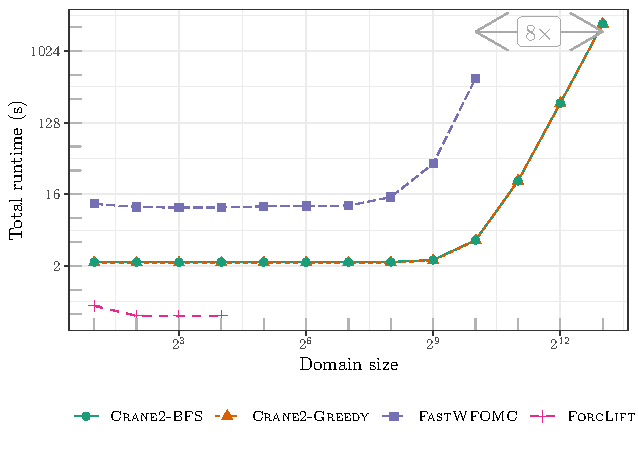
\includegraphics{friends.pdf}
\end{frame}

\begin{frame}{Bijections}
  \centering
  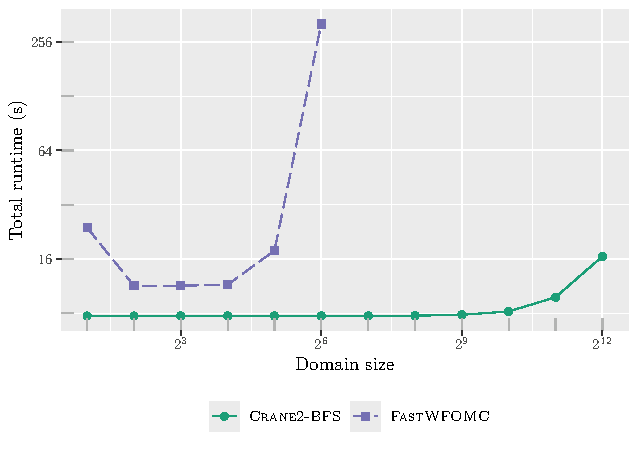
\includegraphics{bijections.pdf}
\end{frame}

\begin{frame}{Functions}
  \centering
  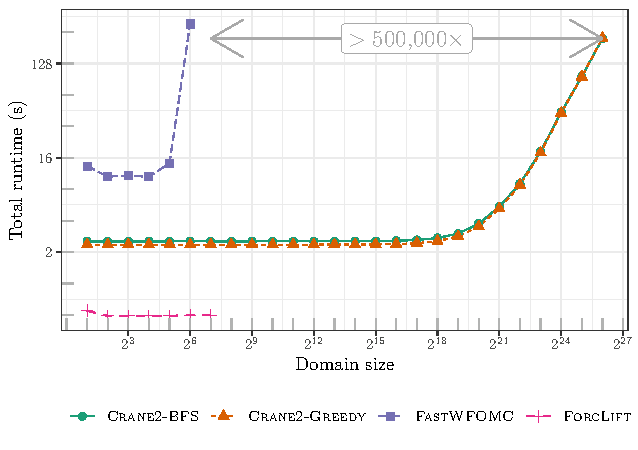
\includegraphics{functions.pdf}
\end{frame}

\begin{frame}{Summary \& Future Work}
  \begin{block}{Contributions}
    \begin{description}
      \item[Completeness:] recursive solutions now come with \alert{base cases}
      \item[Usability:] compilation to C++ programs
      \item[Scalability] compared to other FOMC algorithms
            \begin{itemize}
              \item \numrange{8}{500000} times higher domain sizes
            \end{itemize}
    \end{description}
  \end{block}
  \pause
  \begin{block}{Future Work}
    \begin{itemize}
      \item Support for weighted counting (trivial)
      \item Experiments on a large set of benchmarks
      \item Completeness for fragments of first-order logic
      \item Fine-grained complexity
    \end{itemize}
  \end{block}
  % \vspace{0.5em} \small
  % \begin{itemize}
  %   \item Implementation:
  %         \href{https://github.com/dilkas/crane}{\texttt{github.com/dilkas/crane}}
  %   \item Experimental setup:
  %         \href{https://github.com/dilkas/sat25-ksdm}{\texttt{github.com/dilkas/sat25-ksdm}}
  % \end{itemize}
\end{frame}

\end{document}
